\subsection{KNN Results}

%\mmt{We are only using 5 features, the independent variables: 
%\begin{equation*}
	%\big[m_1,m_2,\chi_1,\chi_2, \rm{SNR}\big]\,.
%\end{equation*}}

\subsubsection{\mmt{Has NS}}
\mmt{The metric we use to compute the distance between neighbors is the \textit{Manhattan} metric (or the Minkowski's $L1$ distance),  which is the distance between two points measured along axes at right angles. Having $p_1(x_1,y_1)$ and $p_2(x_2,y_2)$ the distance will be}
\begin{equation}
	d = |x_1-x_2|+|y_1-y_2|\,.
\end{equation}

\mmt{Moreover, the points are weighted uniformly.  After applying cross-validation,  we get that the optimal number of neighbors is $K_{\rm NS} = 10$, with a mean score $\rm{s_m} = 0:9718355224352762$ and a testing score  $\rm{s_t} = 0.9723828730478842$.} 

%\begin{figure}
%    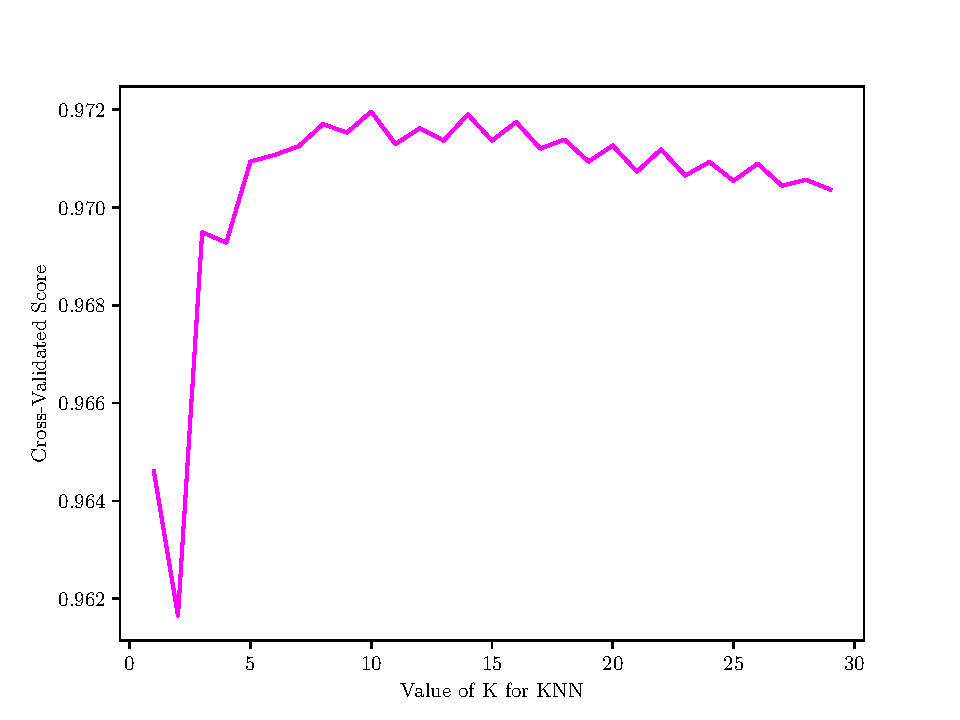
\includegraphics[width = 0.4\textwidth]{CrossValK.pdf}
%    \caption{Score of our KNN model as a function of the number of neighbors. We are considering \textit{HasNS}.}
%    \label{fig:crossvalK}
%\end{figure}
    
\begin{figure}
    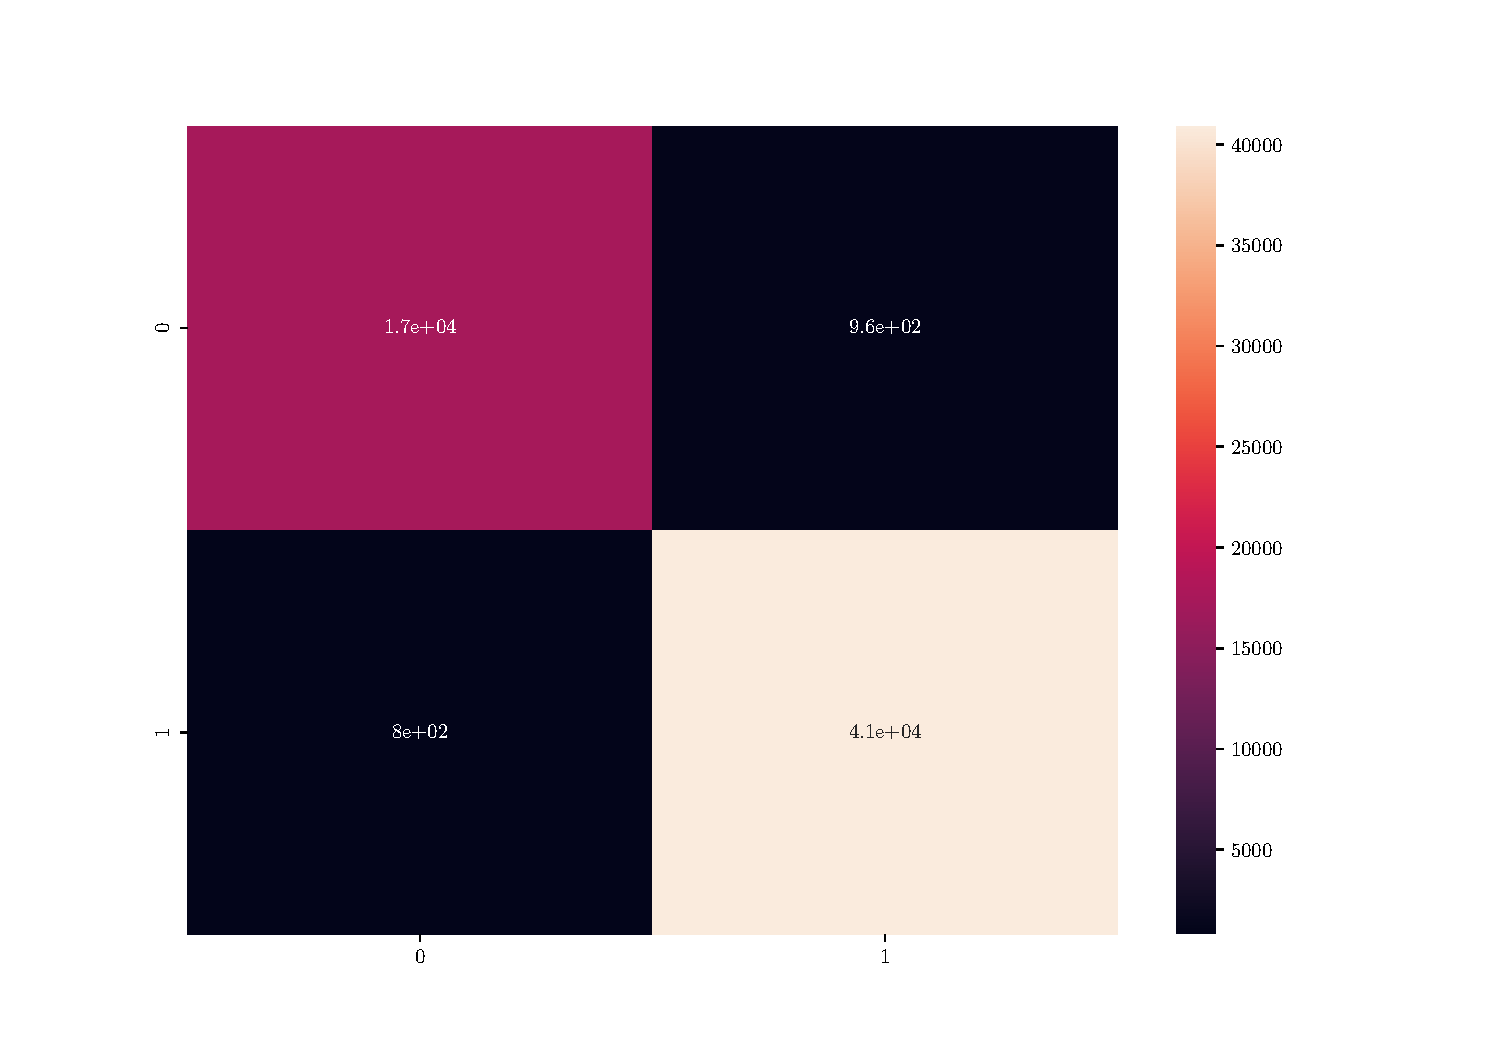
\includegraphics[width=0.45\textwidth]{figs/conf_matrix_NS.pdf}
    \caption{Confusion matrix for our model for \textit{HasNS}, using the independent recovered values. }
    \label{fig:confmat}
\end{figure}

\begin{figure}
    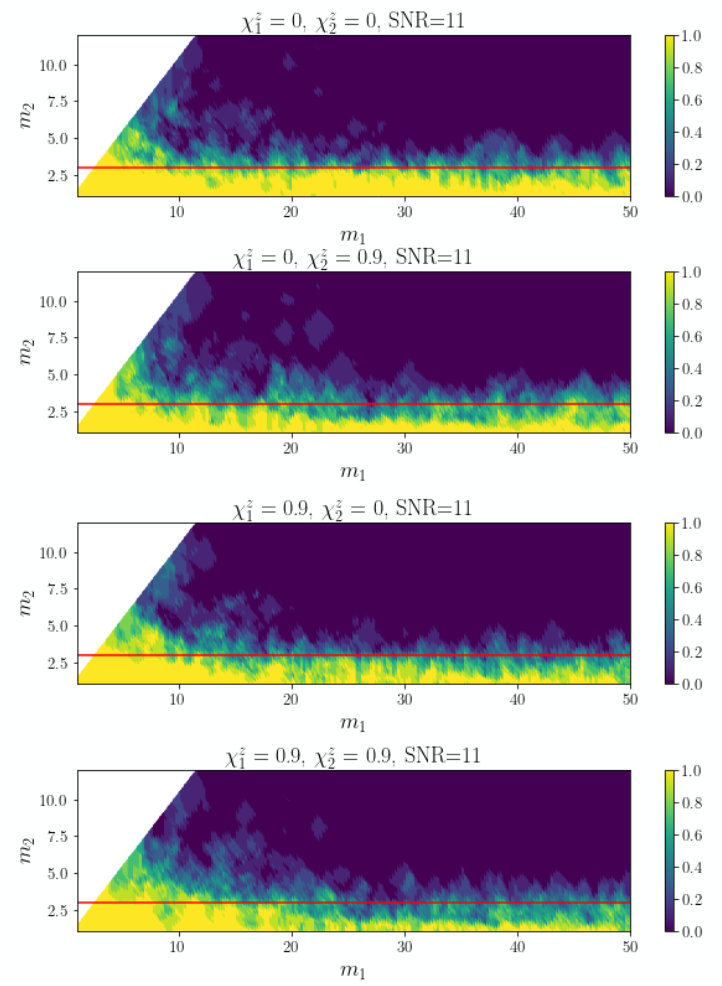
\includegraphics[width = 0.4\textwidth]{plot_fig4_chatt_spins.png}
  %   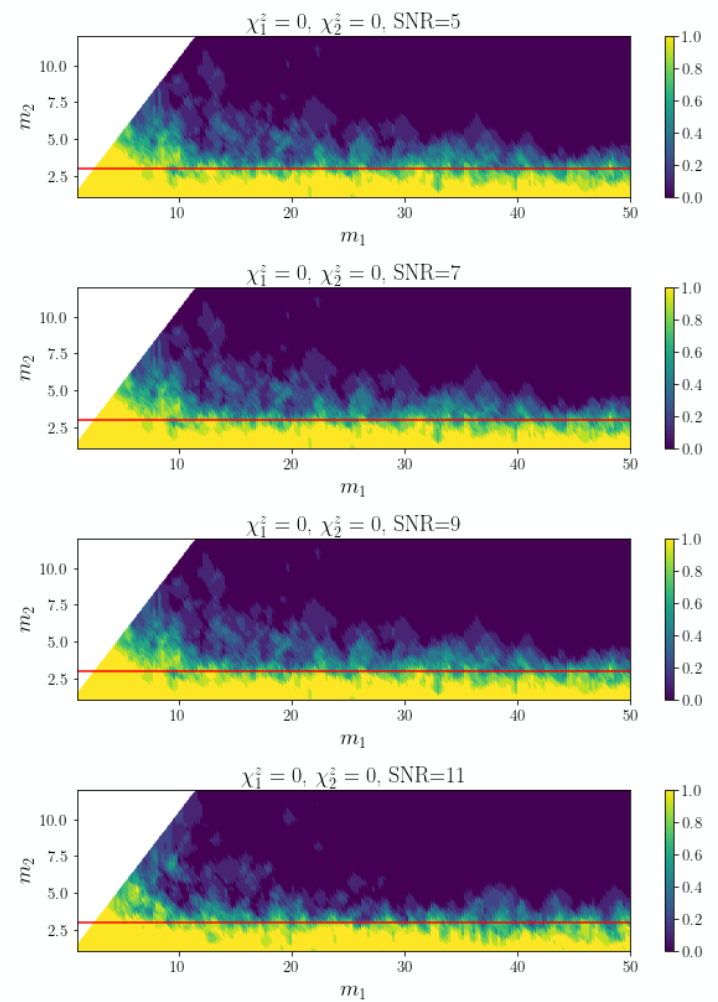
\includegraphics[width = 0.4\textwidth]{/Users/miquelmiravet/Projects/IPAM_LA/ML_group/IPAM2021_ML/algo/classy_KNN/PLOTS_KNN/NS_set/plots_miq/plot_fig4_chatt_snr.png}
    \caption{Probability of having a remnant as a function of the values of the masses. The different panels show the results for different spins. The solid red line depicts the threshold mass for $m_2$.}
    \label{fig:m1m2}
\end{figure}

\begin{figure}
	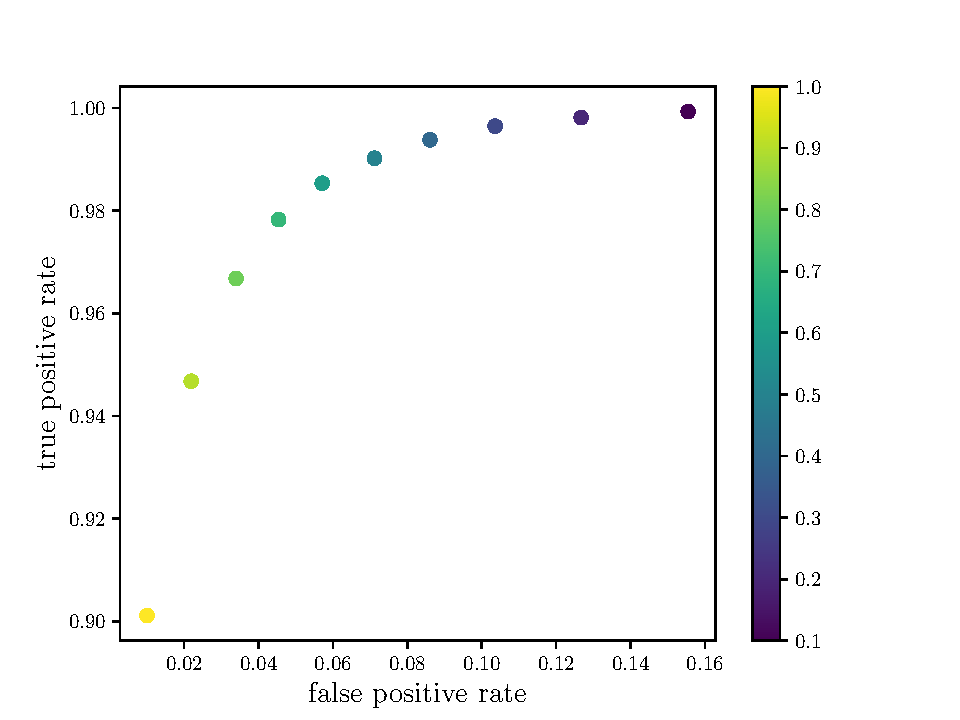
\includegraphics[width =0.4\textwidth]{ROCplot.pdf}
    \caption{Relation of the true and false positive rates as a function of the threshold applied to make the decision between having or not having a remnant. }
    \label{fig:roc}
\end{figure}

\mmt{In Fig. you can find how the mean score changes with the number of neighbors of the algorithm.  The confusion matrix appears in Fig.~\ref{fig:confmat}, the probability as a function of $m_1$ and $m_2$  is shown in Figs.~\ref{fig:m1m2}, and the true and false positive rates in terms of the threshold probability appear in Fig.~\ref{fig:roc}.}


